\documentclass[a4paper, 12pt]{article}
\usepackage{booktabs}
\usepackage{mathtools}
\usepackage{mathtext}
\usepackage{xfrac}
\renewcommand{\arraystretch}{1.4}
\usepackage{pdfpages}

\usepackage{svg}
\newcommand{\svg}[3][0.7] {
  \begin{figure}[h]
    \begin{center}
      \fontsize{7}{8}\selectfont
      \includesvg[scale=#1]{#2}
      \caption{#3}
    \end{center}
  \end{figure}
}

\usepackage[utf8]{inputenc}
\usepackage[T1]{fontenc}
\usepackage[english,russian]{babel}

\begin{document}
\begin{table}
\centering
\label{tbl:7}
\begin{tabular}{|c|c|c|c|c|c|}
\hline
 & $\nu_n^{т}$, кГц & $\nu_n$, кГц & $\sfrac{a_n}{a_1}$ & $\left(\sfrac{a_n}{a_1}\right)^{т}$ & $\Delta_{\%}\left(\sfrac{a_n}{a_1}\right)$ \\
\hline
1 & 1,0 & 1,0 & 1,000 & 1,000 & 0,0 \\
\cline{1-6}
2 & 2,0 & 2,0 & 0,987 & 0,988 & -0,1 \\
\cline{1-6}
3 & 3,0 & 3,0 & 0,968 & 0,967 & 0,0 \\
\cline{1-6}
4 & 4,0 & 4,0 & 0,938 & 0,939 & -0,2 \\
\cline{1-6}
5 & 5,0 & 5,0 & 0,903 & 0,904 & -0,1 \\
\cline{1-6}
6 & 6,0 & 6,0 & 0,861 & 0,862 & -0,1 \\
\cline{1-6}
7 & 7,0 & 7,0 & 0,812 & 0,814 & -0,1 \\
\cline{1-6}
8 & 8,0 & 8,0 & 0,758 & 0,760 & -0,3 \\
\cline{1-6}
9 & 9,0 & 9,0 & 0,698 & 0,702 & -0,5 \\
\cline{1-6}
10 & 10,0 & 10,0 & 0,637 & 0,639 & -0,4 \\
\cline{1-6}
\hline
\end{tabular}
\end{table}


% \svg{svg/7.svg}{gay}
\begin{table}
\centering
\label{tbl:7}
\begin{tabular}{|c|c|c|c|c|c|}
\hline
 & $T$, мкс & $\sfrac{1}{T},\ мс^{-1}$ & $\delta\nu$, кГц & $\delta_{\delta\nu}$, кГц & $\varepsilon_{\delta\nu}$, \% \\
\hline
1 & 200 & 5,000 & 5,001 & 0,032 & 0,64 \\
\cline{1-6}
2 & 500 & 2,000 & 2,000 & 0,003 & 0,15 \\
\cline{1-6}
3 & 1000 & 1,000 & 1,000 & 0,003 & 0,35 \\
\cline{1-6}
4 & 1500 & 0,667 & 0,667 & 0,002 & 0,25 \\
\cline{1-6}
5 & 2000 & 0,500 & 0,500 & 0,001 & 0,26 \\
\cline{1-6}
6 & 2500 & 0,400 & 0,400 & 0,001 & 0,35 \\
\cline{1-6}
7 & 3000 & 0,333 & 0,333 & 0,001 & 0,17 \\
\cline{1-6}
8 & 3500 & 0,286 & 0,286 & 0,000 & 0,11 \\
\cline{1-6}
9 & 4000 & 0,250 & 0,250 & 0,001 & 0,30 \\
\cline{1-6}
10 & 4500 & 0,222 & 0,222 & 0,001 & 0,34 \\
\cline{1-6}
11 & 5000 & 0,200 & 0,200 & 0,001 & 0,30 \\
\cline{1-6}
\hline
\end{tabular}
\end{table}


\svg{svg/10.svg}{gay}

\begin{table}
\centering
\label{tbl:7}
\begin{tabular}{|c|c|c|c|c|}
\hline
 & 1 & 2 & 3 & 4 \\
\hline
$\nu_0$, кГц & 50 & 75 & 50 & 50 \\
\cline{1-5}
$T$, мс & 1 & 1 & 2 & 1 \\
\cline{1-5}
$N$ & 5 & 5 & 5 & 10 \\
\cline{1-5}
$\Delta\nu$, кГц & 20,025 & 30,024 & 20,034 & 9,992 \\
\cline{1-5}
$\delta_{\Delta\nu}$, кГц & 0,016 & 0,018 & 0,005 & 0,022 \\
\cline{1-5}
$\varepsilon_{\Delta\nu}$, \% & 0,08 & 0,06 & 0,03 & 0,22 \\
\cline{1-5}
$\delta\nu$, кГц & 1,0001 & 1,0001 & 0,5000 & 1,0000 \\
\cline{1-5}
$\delta_{\delta\nu}$, кГц & 0,0008 & 0,0006 & 0,0004 & 0,0009 \\
\cline{1-5}
$\varepsilon_{\delta\nu}$, \% & 0,08 & 0,06 & 0,08 & 0,09 \\
\cline{1-5}
\hline
\end{tabular}
\end{table}


\begin{table}
\centering
\label{tbl:7}
\begin{tabular}{|c|c|c|c|c|c|c|c|}
\hline
 & $m$, \% & $a_{\mathrm{base}}$, мВ & $\varepsilon_{a_{\mathrm{base}}}$, \% & $a_{\mathrm{side}}$, мВ & $\varepsilon_{a_{\mathrm{side}}}$, \% & $a_{\mathrm{side}} / a_{\mathrm{base}}$, \% & $\varepsilon_{(a_{\mathrm{side}} / a_{\mathrm{base}})}$, \% \\
\hline
1 & 10 & 704,59 & 0,006 & 35,10 & 0,065 & 4,982 & 0,066 \\
\cline{1-8}
2 & 15 & 705,81 & 0,005 & 52,79 & 0,038 & 7,479 & 0,038 \\
\cline{1-8}
3 & 30 & 705,53 & 0,005 & 105,74 & 0,024 & 14,987 & 0,024 \\
\cline{1-8}
4 & 45 & 705,18 & 0,004 & 158,74 & 0,018 & 22,511 & 0,018 \\
\cline{1-8}
5 & 60 & 705,05 & 0,005 & 211,71 & 0,020 & 30,027 & 0,020 \\
\cline{1-8}
6 & 75 & 704,78 & 0,004 & 264,62 & 0,017 & 37,546 & 0,018 \\
\cline{1-8}
7 & 90 & 704,62 & 0,004 & 317,35 & 0,014 & 45,038 & 0,015 \\
\cline{1-8}
8 & 100 & 704,71 & 0,011 & 353,44 & 0,018 & 50,154 & 0,021 \\
\cline{1-8}
\hline
\end{tabular}
\end{table}


\svg{svg/22.svg}{gay}
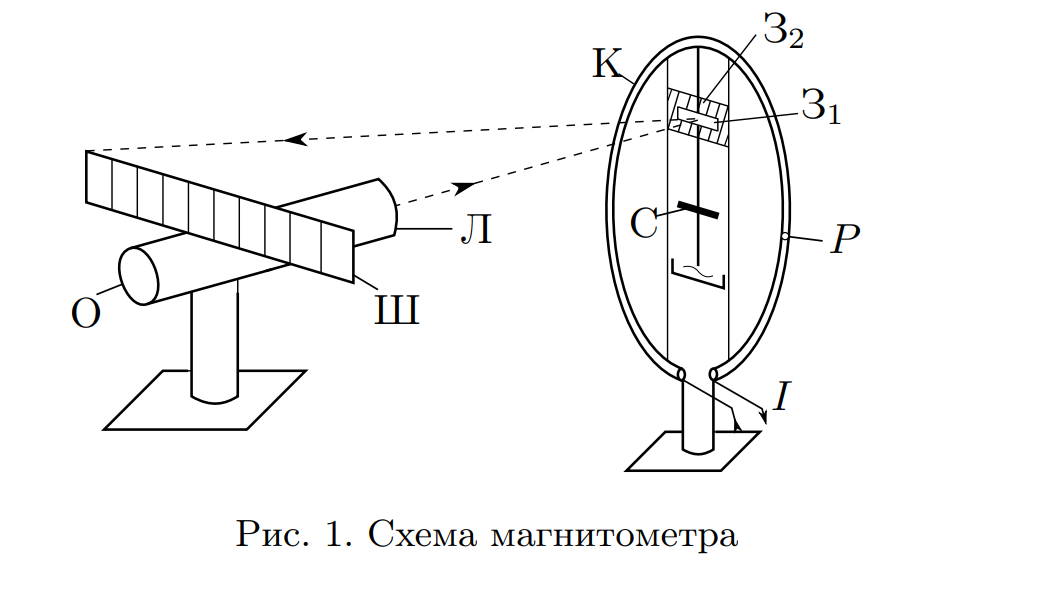
\includepdf[pages=-]{data/1.pdf}
\begin{table}
\centering
\label{tbl:7}
\begin{tabular}{|c|c|c|c|c|c|c|c|c|c|}
\hline
 & $\nu$, кГц & $\delta_{\nu}$, кГц & $a^0$, мВ & $a^{\mathrm{f}}$, мВ & $K$, \% & $\sfrac{1}{K^2}$ & $\delta_{\sfrac{1}{K^2}}$ & $\omega^2 \cdot 10^{-6}$ & $\delta_{\omega^2} \cdot 10^{-6}$ \\
\hline
1 & 0,33283 & 0,00008 & 270,2 & 36,50 & 13,51 & 55 & 2 & 4,373 & 0,002 \\
\cline{1-10}
2 & 0,66681 & 0,00000 & 267,6 & 18,16 & 6,79 & 217 & 8 & 17,553 & 0,000 \\
\cline{1-10}
3 & 0,99949 & 0,00004 & 262,3 & 11,37 & 4,33 & 532 & 20 & 39,438 & 0,003 \\
\cline{1-10}
4 & 1,33362 & 0,00000 & 255,1 & 8,56 & 3,36 & 887 & 32 & 70,214 & 0,000 \\
\cline{1-10}
5 & 1,66641 & 0,00007 & 246,0 & 7,68 & 3,12 & 1026 & 34 & 109,629 & 0,010 \\
\cline{1-10}
6 & 2,00031 & 0,00006 & 235,0 & 5,99 & 2,55 & 1541 & 49 & 157,963 & 0,010 \\
\cline{1-10}
7 & 2,33337 & 0,00010 & 222,6 & 5,07 & 2,28 & 1929 & 58 & 214,946 & 0,018 \\
\cline{1-10}
\hline
\end{tabular}
\end{table}


\svg{svg/28.svg}{gay}
\svg{svg/28_linear.svg}{gay}
\end{document}
~/hw/gphlab/3.6.1/